\documentclass{article}

\usepackage[utf8]{inputenc}
\usepackage[ngerman]{babel}
\usepackage{amssymb}
\usepackage{amsmath}

\usepackage{graphicx}

% Pseudocode
\usepackage{algorithm}
\usepackage[noend]{algpseudocode}

\setlength{\parindent}{0in}

\newcommand{\uebungsGruppe}{1}
\newcommand{\zettelNummer}{1}
\newcommand{\studierenderEins}{Eli Kogan-Wang (7251030)}
\newcommand{\studierenderZwei}{David Noah Stamm (7249709)}
\newcommand{\studierenderDrei}{Daniel Heins (7213874)}
\newcommand{\studierenderVier}{Tim Wolf (7269381)}

\newcounter{AufgabenCounter}
\setcounter{AufgabenCounter}{1}
\newcounter{TeilaufgabenCounter}
\newenvironment{aufgabe}{\section*{Aufgabe \theAufgabenCounter}\setcounter{TeilaufgabenCounter}{1}}{\stepcounter{AufgabenCounter}}
\newenvironment{teilaufgabe}{\paragraph*{\alph{TeilaufgabenCounter})}}{\stepcounter{TeilaufgabenCounter}}

\renewcommand{\to}{\textnormal{ to }}
\newcommand{\bigO}{\mathcal{O}}

\newcommand{\qed}{\hfill$\square$}

\begin{document}

\title{Datenstrukturen und Algorithmen \\ Heimübung \zettelNummer{}}
\author{\studierenderEins{} \\
  \studierenderZwei{} \\
  \studierenderDrei{} \\
  \studierenderVier{}}

\maketitle

\begin{aufgabe}

  Pow in linearer Zeit:
  \begin{algorithm}[H]
    \caption{\textsc{PowLin}($x, n$)}
    \begin{algorithmic}[1]
      \State $result \gets 1$ \Comment{$O(1)$}
      \While{$n > 0$} \Comment{$\sigma_{i=1}^kT(I)$}
      \If{$n \mod 2 = 1$} \Comment{$O(1)$}
      \State $result \gets result \cdot x$ \Comment{$O(1)$}
      \EndIf
      \State $x \gets x \cdot x$ \Comment{$O(1)$}
      \State $n \gets (n - (n \mod 2)) / 2$ \Comment{$O(1)$}
      \EndWhile
      \State \textbf{Return} $result$ \Comment{$O(1)$}
    \end{algorithmic}
  \end{algorithm}

  \textbf{Schleifeninvariante:}

  $$I(n):= result_n \cdot (x_n)^{n} = (x_{orig})^{n_{orig}}$$

  \textbf{Korrektheit:}

  \textbf{Initialisierung:}

  $n = n_{orig}$\\
  $x = x_{orig}$\\
  $result = 1$
  $$result\cdot x^n = (x_{orig})^{n_{orig}}$$

  \textbf{Erhaltung:}

  Gegeben sei für die $i$-te Iteration:

  $$I(n_i) := result_{n_i} \cdot (x_{n_i})^{n_{n_i}} = (x_{orig})^{n_{orig}}$$

  Es gilt: $I(n_i)$.

  Nun ist zu zeigen:

  $$I(n_{i+1}) = result_{n_{i+1}} \cdot (x_{n_{i+1}})^{n_{n_{i+1}}} = (x_{orig})^{n_{orig}}$$

  Durchführung:

  $result_{n_{i+1}}$
  $$= \begin{cases}
      result_{n_{i+1}}                   & \text{falls } n_{n_{i+1}} \mod 2 = 0 \\
      result_{n_{i+1}} \cdot x_{n_{i+1}} & \text{falls } n_{n_{i+1}} \mod 2 = 1 \\
    \end{cases}
    = result_{n_i} \cdot x^{n_{n_i} \mod 2}$$
  $$x_{n_{i+1}}= x_{n_i} \cdot x_{n_i} = x_{n_i}^{2}$$
  $$n_{n_{i+1}} = \frac{(n_{n_i} - (n_{n_i} \mod 2))}{2}$$


  $$\begin{aligned}
      LHS & = result_{n_{i+1}} \cdot (x_{n_{i+1}})^{n_{n_{i+1}}}                                                   \\
          & = (result_{n_i} \cdot x^{n_{n_i} \mod 2}) \cdot (x_{n_i}^{2})^{\frac{(n_{n_i} - (n_{n_i} \mod 2))}{2}} \\
          & = result_{n_i} \cdot x^{n_{n_i} \mod 2} \cdot ((x_{n_i}^{2})^{\frac12})^{(n_{n_i} - (n_{n_i} \mod 2))} \\
          & = result_{n_i} \cdot x^{(n_{n_i} \mod 2)} \cdot x_{n_i}^{n_{n_i} - (n_{n_i} \mod 2)}                   \\
          & = result_{n_i} \cdot (x_{n_i})^{n_{n_i}}                                                               \\
          & \overset{Annahme}{=} (x_{orig})^{n_{orig}}
    \end{aligned}$$

  \textbf{Laufzeit:}

  Potentialfunktion: $\Psi(n) = \log(n)$\\
  Wir brechen ab, wenn $n \not > 0$ also, wenn $\log(n) \not > 1$\\
  Da $n_{i+1} = \frac{(n_{i} - (n_{i} \mod 2))}{2}$:\\
  $\Psi(n_{i+1}) \leq \Psi(n_i)-1$

  Damit: $k\in O(\frac{\Psi(n)}{1}) = O(\log(n))$\\
  $O(1)+O(\log(n))+O(1) = O(\log(n))$\\
  Damit hat der Algorithmus die Laufzeit $O(\log(n))$

\end{aufgabe}

\begin{aufgabe}
  \begin{teilaufgabe}
    \begin{algorithm}
      \caption{\textsc{NonRecMergeSort}($A[1,\dots,2^k]$)}

      \begin{algorithmic}
        \For{$i \gets 1$ up to $k$}
        \For{$j \gets 0$ up to $2^{k-i} -1$}
        \State $Merge(A, 2^i\cdot j+1, 2^i\cdot j+(2^{i-1})+1, 2^i\cdot (j+1))$
        \EndFor
        \EndFor
      \end{algorithmic}
    \end{algorithm}

  \end{teilaufgabe}
  \begin{teilaufgabe}
    Hilfsdefinitionen:

    $$Sorted(A[n,\dots,m]) := \forall i \in [n,m): A[i] \leq A[i+1]$$

    Invarianten:

    $I(i,j) := \forall l \in [0:2^{k-i}-1-j): Sorted(A[2^{i}\cdot l,\dots,2^{i}\cdot (l + 1) - 1])$

    $I(i) := \forall m \in [1:i): \forall j \in [0:2^{k-i}-1]: Sorted(A[2^{i}\cdot j,\dots,2^{i}\cdot (j + 1) - 1])$
  \end{teilaufgabe}

\end{aufgabe}

\begin{aufgabe}

  % Image 2022-04-29-DuA_3.JPG


  \noindent\makebox[\textwidth]{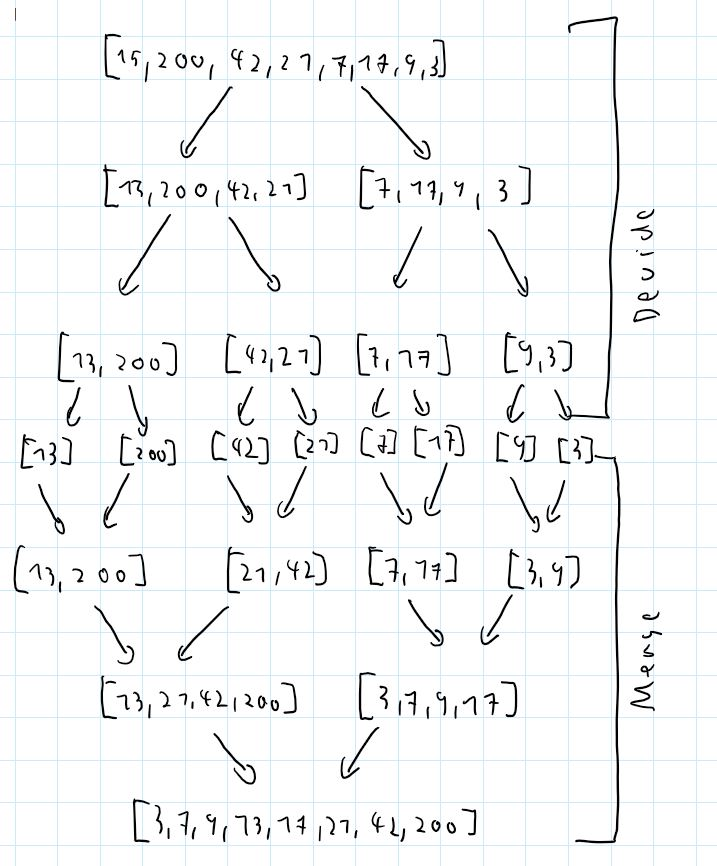
\includegraphics[width=\textwidth]{2022-04-29-DuA_3.JPG}}
\end{aufgabe}

\end{document}

